\documentclass[10pt]{report}

\usepackage[T1]{fontenc}
\usepackage[utf8]{inputenc}
\usepackage[french]{babel}
\usepackage{amsmath}
\usepackage{amsfonts}
\usepackage{amssymb}
\usepackage{graphicx}

\title{INGI2261- AI - Project 2}
\author{Jacquet Charles - 27811200 \\ Degryse Baptiste - 27641200\\ Groupe 34}
\date\today
\begin{document}
\maketitle
\section*{First set of questions}
\subsection*{1) Heuristic}
The heuristic can simple be the Manhattan distance between the guy and the goal.
It's admissible beacuse if there is no wall, the estimation of the solution by the heuristic is actually the real value. And in other case the heuristic value is underestimated.

\subsection*{2) uniform-cost graph search}
\begin{center}
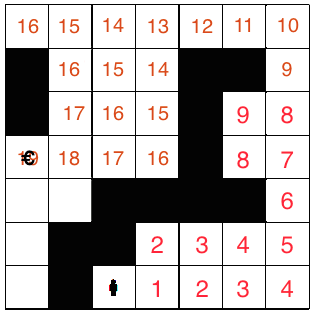
\includegraphics[scale=0.5]{uniform-cost.png}
\end{center}

\subsection*{3) A* graph search}
\begin{center}
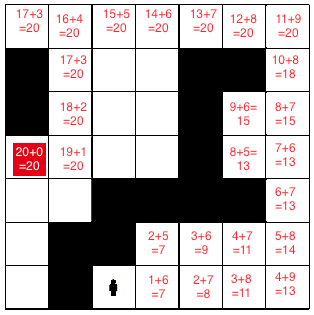
\includegraphics[scale=0.5]{A_star.png}
\end{center}

\section*{Second set of questions}
\subsection*{Other dead-end ?}
We first thought about the case where a line was made, creating a place without any goal where the perso can’t go. But after thinking about it, testing this case was not an improvement at all. Actually it was quite the opposite because in that case, only one or two expand are needed to our algorithme to understand by other ways (like dead-end) that iss not a possible way. So checking that all the time is a lot of calculation for nearly nothing.

\subsection*{The importance of searching dead-state}
It’s really important because when a path cannot lead to a solution, we have to delete it as quickly as possible because the program can take a lot of time expanding these nodes for nothing. In order to do that, we looked for four dead-end position, when the box is in a corner (and the 3 other symmetric corner).

\subsection*{Our heuristic}
We have decided to have the simplest heuristic as possible. We first tried to have only the heuristic on the Manhattan distance between boxes and there nearest free box goal (‘.’).
Then, we tried to improve it by adding an heuristic on the distance for the person but it was not a good idea at all! Yes it did what we wanted to but we saw that it was not always the optimal solution. Moreover, it was a lot to calculate at each time. So we came back to our first choice which is admissible because in the best case, we have that the estimate distance is the same as said by the heuristic (if the perso has just to push the box without any direction modification). In other case, it underestimates the path. \\
Then it had to be consistent, thus, when the perso moves from n to n' we must have :
$$h(n)\leq c(n,a,n') + h(n')$$
to see that our heuristic is consistency the only possible cases are (cost is 1 for each moves):
\begin{itemize}
\item h(n')=h(n)+cost = h(n)+1 (perso moved but didn't push any box)
\item h(n')=h(n)+1+ cost =h(n)+2 (perso moved push a box)
\item h(n')=h(n)-1 + cost = h(n) (perso moved push a box)
\end{itemize}
So we see that the consistency equation is satisfied.

\subsection*{The implementation is on the Inginious platform}
\subsection*{A* (informed search) vs uniform-cost Search() (uninformed search)}

\begin{table}[h!]
\centering
\caption{uninformed vs informed search graph}
\label{uninformedVsInformed}
\begin{tabular}{lll}
                 & uninformed search (breadth first graph search) & informed search (A*) \\
sokoInst01-time  & 0.34653                                        & 0.01542              \\
sokoInst01-node  & 2883                                           & 114                  \\
sokoInst02-time  & 1.07803                                        & 0.88283              \\
sokoInst02-node  & 6990                                           & 4967                 \\
sokoInst07-time  & 1.07651                                        & 0.61504              \\
sokoInst07-node  & 4252                                           & 2417                 \\
sokoInst08-time  & 1.31147                                        & 0.83353              \\
sokoInst08-node  & 6403                                           & 3570                 \\
sokoInst015-time & 13.91409                                       & 0.64684              \\
sokoInst015-node & 67875                                          & 2799                
\end{tabular}
\end{table}

With these results (cfr Table \ref{uninformedVsInformed}), we clearly see that informed search is more efficient than the other one, it takes less time and visit less states. It means that the heuristic is really helping in the choose of which state to expand first.
\section*{Performance without dead-end detection}

\begin{table}[h!]
\centering
\caption{My caption}
\label{dead-end}
\begin{tabular}{lll}
                 & A* without dead-end detection & informed search (A*) \\
sokoInst01-time  & 0.0153                        & 0.01542              \\
sokoInst01-node  & 114                           & 114                  \\
sokoInst02-time  & 2.86740                       & 0.88283              \\
sokoInst02-node  & 15613                         & 4967                 \\
sokoInst07-time  & 1.51757                       & 0.61504              \\
sokoInst07-node  & 5497                          & 2417                 \\
sokoInst08-time  & 1.4537                        & 0.83353              \\
sokoInst08-node  & 6297                          & 3570                 \\
sokoInst015-time &  time-out                             & 0.64684              \\
sokoInst015-node & 204053                        & 2799                
\end{tabular}
\end{table}

We can see on the Table \ref{dead-end} that except for the first case, we have to visit twice more nodes when we are not checking for dead-ends!
\end{document}
